\section{Introduction}
\label{sec:introduction}

% state the learning objective 
The objective of this laboratory assignment is to study a circuit with four meshes containing a capacitor, a sinusoidal voltage source $v_s$ and two linearly dependent sources: a voltage controlled current source $I_b$ and a current controlled voltage source $V_d$. The circuit also contains seven resistors from $R_1$ to $R_7$ as it is shown in Figure~\ref{fig:Circuit_Base}.
The values for the caracteristics of this components, apart from $I_d$ and $V_b$ and including $v_s$, $C$, $K_b$ and $K_d$, are given by Python and are:

\begin{table}[h]
  \centering
 \begin{tabular}{|l|r|}
    \hline    
    {\bf Name} & {\bf Value [A, V, S, $\Omega$ or F]} \\ \hline
    \input{../mat/DATA_tab}
  \end{tabular}
  \caption{Variables in the Nodal Method. A variable preceded by @ is of type {\em current} and expressed in Ampere; variables preceded by \# is of type {\em resistance} and expressed in Ohm; variables preceded by § is of type {\em conductance} and expressed in Seimens; ariables preceded by \& is of type {\em capacitance} and expressed in Farad; other variables are of type {\em voltage} and expressed in Volt.}
  \label{tab:Enunciado}
\end{table}

In Section~\ref{sec:analysis}, a theoretical analysis of the circuit is
presented. In Section~\ref{sec:simulation}, the circuit is analysed by
simulation, and the results are compared to the theoretical ones obtained in
Section~\ref{sec:analysis}. The conclusions of this study are outlined in
Section~\ref{sec:conclusion}.

\begin{figure}[h] \centering
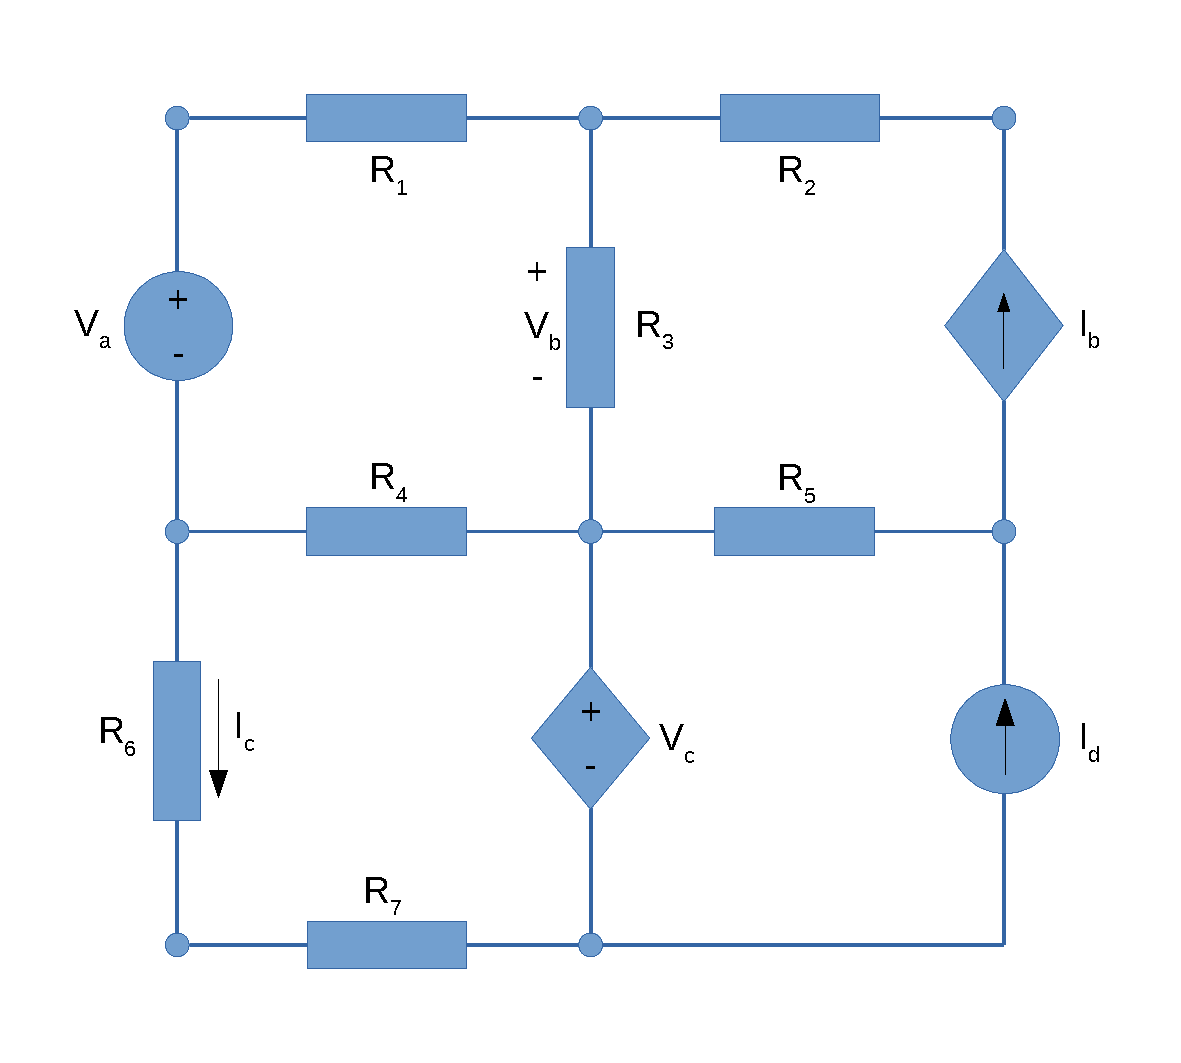
\includegraphics[width=0.5\linewidth]{Circuit.pdf}
\caption{Circuit analysed.}
\label{fig:Circuit_Base}
\end{figure}